\documentclass{article}
\usepackage[preprint]{colm2026_conference}

\usepackage{microtype}
\usepackage{hyperref}
\usepackage{url}
\usepackage{booktabs}
\usepackage{graphicx}
\usepackage{amsmath}
\usepackage{amssymb}
\usepackage{multirow}
\usepackage{subcaption}
\usepackage{xcolor}
\usepackage{tikz}
\usetikzlibrary{arrows.meta, positioning, shapes.geometric, fit, calc}

\definecolor{darkblue}{rgb}{0, 0, 0.5}
\hypersetup{colorlinks=true, citecolor=darkblue, linkcolor=darkblue, urlcolor=darkblue}

\title{ComSense Circuits: Mechanistic Interpretability of\\
Commonsense Reasoning Failures in Large Language Models}

\author{%
  \begin{tabular}[t]{c}\bf Zhizhong Sang \\ \texttt{zhizhongs@uchicago.edu}\end{tabular} \hfill
  \begin{tabular}[t]{c}\bf Haoxiang Xiong \\ \texttt{haoxiang@uchicago.edu}\end{tabular} \hfill
  \begin{tabular}[t]{c}\bf Ruotian Wang \\ \texttt{ruotian2003@uchicago.edu}\end{tabular} \\
  \\[0.5em]
  \textbf{Advisor:} Darin Keng
}

\newcommand{\fix}{\marginpar{FIX}}
\newcommand{\new}{\marginpar{NEW}}

\begin{document}

\maketitle

\begin{abstract}
Large language models routinely fail at commonsense reasoning tasks that seem trivial to humans, yet the internal mechanisms underlying these failures remain poorly understood.
We present a systematic mechanistic interpretability study of commonsense reasoning failures in Qwen3-8B, evaluated on the Com2Sense dataset of 2,390 True/False statements organized in complementary pairs.
Starting from 611 \emph{asymmetric pairs}---where the model answers one member of a complementary pair correctly and the other incorrectly---we conduct a five-phase investigation combining residual-stream probing, activation patching, head-level analysis, mean-ablation, logit-lens trajectory analysis, and MLP/attention sublayer decomposition.
Our central finding is that commonsense reasoning failures are \emph{fundamentally distributed}: no single layer or attention head is sufficient (0\% flip rate under activation patching across 18 layers and 160 head-layer combinations) or necessary (maximum 1\% flip rate under mean-ablation of 17 candidate heads) for correct commonsense predictions.
Probing accuracy plateaus at ${\sim}59$\% even with optimal regularization, and layer-by-layer logit-lens trajectories reveal that 76.5\% of incorrect predictions are already directionally wrong at layer~0, with the wrong answer consolidating stably around layer~20.
These results contrast sharply with prior mechanistic work on factual recall, where localized circuits yield high flip rates, and suggest that commonsense reasoning requires a fundamentally different diagnostic and repair strategy than surgical circuit-level intervention.
\end{abstract}

%=============================================================================
\section{Introduction}
\label{sec:intro}
%=============================================================================

Large language models achieve impressive scores on many commonsense benchmarks, yet still fail on surprising cases that seem trivial to humans~\citep{davis2023commonsense}.
Understanding \emph{why} these failures occur---and where in the model they originate---is a central challenge for mechanistic interpretability.
Prior work has successfully localized factual recall circuits in GPT-2 and related models~\citep{wang2022interpretability, geva2023dissecting, meng2022locating}, demonstrating that specific attention heads and MLP layers mediate factual associations with high patching flip rates.
Commonsense reasoning, however, presents a structurally different challenge: unlike factual associations that can be attributed to specific (subject, relation, object) triples, commonsense judgments require integrating world knowledge, physical intuition, temporal reasoning, and social understanding that may be encoded in a distributed, non-local manner.

We ask three questions:
\begin{enumerate}
    \item Are commonsense reasoning failures \textbf{localized} to specific layers or attention heads, or are they \textbf{distributed} across the network?
    \item Do failures reflect a \textbf{knowledge-retrieval} deficit (the model never encodes the relevant knowledge) or an \textbf{inference} failure (knowledge is present but not used correctly)?
    \item Are the failures primarily \textbf{architectural} (the model cannot represent commonsense), \textbf{representational} (it can but doesn't), or \textbf{training-induced} (insufficient training signal)?
\end{enumerate}

To answer these questions, we evaluate Qwen3-8B~\citep{qwen3} on Com2Sense~\citep{singh2021com2sense}, a benchmark of 2,390 True/False statements organized in complementary pairs (e.g., ``Rocks make a good pillow'' paired with ``Rocks are too hard to sleep on'').
The model achieves 70.25\% overall accuracy, identifying 611 \emph{asymmetric pairs} where it answers one member correctly and the other incorrectly.
We use 200 of these pairs---selected for high wrong-answer confidence---as the substrate for mechanistic analysis across five complementary techniques: residual-stream probing, activation patching (layer-level, head-level, and sublayer-level), head-level probing, mean-ablation, and logit-lens trajectory analysis, all implemented via TransformerLens~\citep{nanda2022transformerlens}.

Our main finding is that commonsense failures are \emph{fundamentally distributed}: layer-level and head-level patching produce 0\% prediction flips, sublayer-level (attention or MLP) patching achieves at most 1.5\%, probing any individual component achieves only ${\sim}59$\% accuracy, and logit-lens trajectories reveal a complex multi-stage failure process beginning at the earliest layers.
This distinguishes commonsense from factual recall and has implications for how alignment-relevant commonsense deficits can be diagnosed and repaired.

%=============================================================================
\section{Background}
\label{sec:background}
%=============================================================================

Modern transformer language models~\citep{Vaswani+2017} process input through a sequence of layers, each containing an attention sublayer and a feed-forward (MLP) sublayer whose outputs are added to a \emph{residual stream}---the running sum of all sublayer contributions that carries information forward through the network~\citep{elhage2021mathematical}.
Mechanistic interpretability seeks to understand model behavior by analyzing this residual stream and the individual components that write to it.

Several tools from this literature are central to our study.
\emph{Linear probing}~\citep{belinkov2022probing} trains a classifier on residual-stream vectors to test whether a given property (e.g., the correct answer) is linearly decodable at each layer.
\emph{Activation patching}~\citep{meng2022locating, wang2022interpretability} replaces a component's activation from one input with that from another, testing whether the component is \emph{sufficient} to change the model's prediction; \emph{mean-ablation} replaces it with the population mean to test \emph{necessity}.
The \emph{logit lens}~\citep{nostalgebraist2020logitlens} projects the residual stream at each layer through the model's unembedding matrix, revealing how the predicted output token evolves layer by layer.

Prior mechanistic work has shown that \emph{factual recall} is remarkably localized: \citet{geva2023dissecting} find that patching specific layers flips factual predictions 30--60\%+ of the time, and \citet{meng2022locating} show that editing a small number of MLP layers can reliably alter stored facts.
Whether commonsense reasoning---which requires integrating world knowledge, temporal reasoning, and social understanding---admits similar localization is the question we investigate.

%=============================================================================
\section{Methodology}
\label{sec:methods}
%=============================================================================

Figure~\ref{fig:pipeline} provides an overview of our five-phase experimental pipeline.

\begin{figure*}[t]
\centering
\resizebox{\textwidth}{!}{%
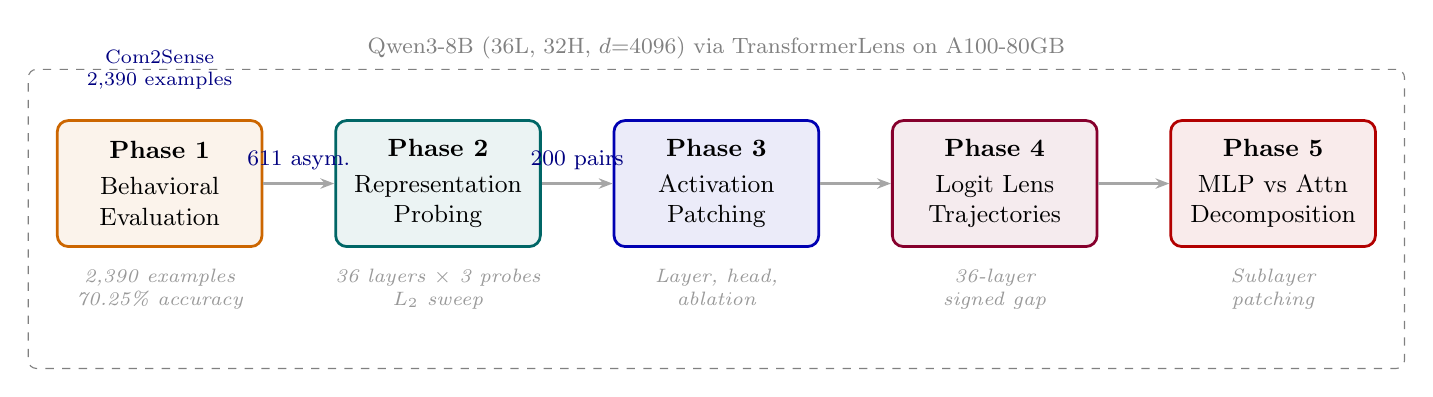
\begin{tikzpicture}[
    node distance=0.4cm and 0.25cm,
    phase/.style={rectangle, rounded corners=4pt, draw=#1, fill=#1!8, line width=1pt,
                  minimum height=1.6cm, minimum width=2.6cm, align=center, font=\small},
    arrow/.style={-{Stealth[length=5pt]}, line width=0.8pt, color=gray!70},
    sublabel/.style={font=\scriptsize\itshape, text=gray!80, align=center},
    datalabel/.style={font=\scriptsize, text=darkblue, align=center},
]

% Phase 1
\node[phase=orange!80!black] (p1) {
    \textbf{Phase 1}\\[2pt]
    Behavioral\\Evaluation
};
\node[sublabel, below=0.15cm of p1] (p1sub) {2,390 examples\\70.25\% accuracy};

% Phase 2
\node[phase=teal!80!black, right=0.9cm of p1] (p2) {
    \textbf{Phase 2}\\[2pt]
    Representation\\Probing
};
\node[sublabel, below=0.15cm of p2] (p2sub) {36 layers $\times$ 3 probes\\$L_2$ sweep};

% Phase 3
\node[phase=blue!70!black, right=0.9cm of p2] (p3) {
    \textbf{Phase 3}\\[2pt]
    Activation\\Patching
};
\node[sublabel, below=0.15cm of p3] (p3sub) {Layer, head,\\ablation};

% Phase 4
\node[phase=purple!70!black, right=0.9cm of p3] (p4) {
    \textbf{Phase 4}\\[2pt]
    Logit Lens\\Trajectories
};
\node[sublabel, below=0.15cm of p4] (p4sub) {36-layer\\signed gap};

% Phase 5
\node[phase=red!70!black, right=0.9cm of p4] (p5) {
    \textbf{Phase 5}\\[2pt]
    MLP vs Attn\\Decomposition
};
\node[sublabel, below=0.15cm of p5] (p5sub) {Sublayer\\patching};

% Arrows between phases
\draw[arrow] (p1) -- (p2);
\draw[arrow] (p2) -- (p3);
\draw[arrow] (p3) -- (p4);
\draw[arrow] (p4) -- (p5);

% Data flow labels
\node[datalabel, above=0.25cm of p1] {Com2Sense\\2,390 examples};
\node[datalabel, above=0.05cm of $(p1.east)!0.5!(p2.west)$] {\footnotesize 611 asym.};
\node[datalabel, above=0.05cm of $(p2.east)!0.5!(p3.west)$] {\footnotesize 200 pairs};

% Model box spanning all phases
\node[draw=gray, dashed, rounded corners=3pt, fit=(p1)(p5)(p1sub)(p5sub),
      inner xsep=10pt, inner ysep=18pt, label={[font=\footnotesize, text=gray]above:Qwen3-8B (36L, 32H, $d$=4096) via TransformerLens on A100-80GB}] {};

\end{tikzpicture}
}
\caption{Overview of the five-phase experimental pipeline. Each phase builds on the outputs of the previous: behavioral evaluation identifies asymmetric failure pairs, probing localizes signal to layers 20+, patching and ablation test sufficiency and necessity of individual components, logit lens reveals layer-by-layer prediction trajectories, and sublayer decomposition tests attention vs.\ MLP contributions.}
\label{fig:pipeline}
\end{figure*}

\subsection{Model and dataset}

We use Qwen3-8B (36 layers, 32 heads, $d_\text{model}{=}4096$, $d_\text{head}{=}128$) in TransformerLens on an A100-80GB GPU.
We disable chain-of-thought mode (\texttt{/no\_think}) and evaluate statements by comparing final-position logits for \texttt{True} and \texttt{False}.
Com2Sense is loaded from \texttt{tasksource/com2sense}, with complementary pair assignments from the official GitHub mapping.

\subsection{Asymmetric pair selection}

From 1,195 valid complementary pairs, we identify 611 \emph{asymmetric} pairs where the model answers exactly one member correctly.
For mechanistic analysis, we select 200 pairs: 103 from the time domain, 50 temporal, and 47 social, prioritizing pairs with high-confidence wrong answers (mean confidence 0.896, mean logit gap 2.534) to maximize the signal-to-noise ratio of our interventions.

\subsection{Representation probing}

For each selected example we cache final-token \texttt{hook\_resid\_post} across all 36 layers and train logistic-regression probes with grouped 5-fold cross-validation (both members of each complementary pair are assigned to the same fold to prevent leakage from near-duplicate sentences), probing both correctness and ground truth.
We test both raw features and PCA-50 and sweep $L_2$ regularization over $C \in \{0.001, 0.01, 0.1, 0.5, 1.0, 5.0, 10.0\}$.

\subsection{Activation patching}

For each of 200 pairs and 18 layers (18--35), we cache the correct example's final-token activation, patch it into the incorrect example, and record logit change and flips.
We also patch \texttt{hook\_attn\_out} and \texttt{hook\_mlp\_out} separately.

\subsection{Head-level analysis}

We complement layer patching with head patching on the top five layers by patching effect, head probing over all 576 heads in layers 18--35, and mean-ablation on 17 candidate heads identified from patching and probing.

\subsection{Logit lens}

We project the cached final-token residual stream through the model's final layer norm and unembedding at every layer, recovering a signed logit gap:
\[
\Delta_\ell = \text{logit}[\texttt{True}]_\ell - \text{logit}[\texttt{False}]_\ell
\]
To make trajectories comparable across examples with different ground-truth labels, we sign-correct so that positive values indicate the model supports the ground truth and negative values indicate it supports the wrong answer.

%=============================================================================
\section{Results}
\label{sec:results}
%=============================================================================

\subsection{Phase 1: Behavioral evaluation}

Qwen3-8B achieves \textbf{70.25\% accuracy} on Com2Sense (1,679/2,390 correct).
Table~\ref{tab:accuracy} breaks down performance by domain and scenario.
The model performs best on physical statements (76.27\%) and worst on temporal ones (63.53\%), suggesting that reasoning about temporal order and duration poses a greater challenge than physical-world knowledge for this model.

\begin{table}[t]
\centering
\small
\caption{Accuracy by domain and scenario on Com2Sense (2,390 examples).}
\label{tab:accuracy}
\begin{tabular}{lrr}
\toprule
\textbf{Subset} & \textbf{Accuracy} & \textbf{Count} \\
\midrule
Overall & 70.25\% & 2,390 \\
\midrule
Physical & 76.27\% & 805 \\
Social & 68.77\% & 794 \\
Time & 66.60\% & 536 \\
Temporal & 63.53\% & 255 \\
\midrule
Causal & 70.53\% & 1,198 \\
Comparison & 70.02\% & 804 \\
Comparative & 70.03\% & 387 \\
\bottomrule
\end{tabular}
\end{table}

\paragraph{False-bias.}
Of the 611 asymmetric pairs, \textbf{73.6\% involve the model failing on a True statement}---the model systematically defaults to ``False'' when uncertain.
Table~\ref{tab:false_bias} shows this bias is pervasive across all domains, peaking at 87.0\% in social-causal scenarios.
This directional asymmetry is not a generic difficulty effect: it reveals a systematic inference default where the model preferentially rejects statements rather than accepting them under uncertainty.

\begin{table}[t]
\centering
\small
\caption{False-bias in asymmetric failures: percentage of failures where the model incorrectly rejects a True statement.}
\label{tab:false_bias}
\begin{tabular}{lrrr}
\toprule
\textbf{Domain / Scenario} & \textbf{Failed TRUE} & \textbf{Total} & \textbf{\% TRUE} \\
\midrule
Overall & 450 & 611 & 73.6\% \\
\midrule
Social & 162 & 208 & 77.9\% \\
Physical & 125 & 169 & 74.0\% \\
Time & 111 & 157 & 70.7\% \\
Temporal & 52 & 77 & 67.5\% \\
\midrule
Social-causal & 87 & 100 & 87.0\% \\
Physical-causal & 73 & 95 & 76.8\% \\
Time-causal & 57 & 80 & 71.2\% \\
Temporal-comparative & 22 & 36 & 61.1\% \\
\bottomrule
\end{tabular}
\end{table}

\subsection{Phase 2: Representation probing}

\paragraph{Layer-wise probing.}
Figure~\ref{fig:probing} (left) shows per-layer probing accuracy across three configurations.
All probes are at chance (${\sim}50$\%) through layers 0--19 and rise sharply from layer~20 onward, peaking in the 23--34 range.
Table~\ref{tab:probing} summarizes the original probe results.

\begin{table}[t]
\centering
\small
\caption{Phase~2 probing results (original $C{=}1.0$ and $L_2$-corrected). ``Layer'' column shows best layer before $\to$ after regularization correction.}
\label{tab:probing}
\begin{tabular}{lcccc}
\toprule
\textbf{Probe} & \textbf{Layer} & \textbf{Original} & \textbf{Best $C$} & \textbf{Corrected} \\
\midrule
Correctness (no PCA) & 32$\to$34 & 54.75\% & 0.001 & 57.50\% \\
Correctness + PCA-50 & 30$\to$23 & 61.00\% & 0.01 & 58.75\% \\
Ground truth + PCA-50 & 31$\to$32 & 60.00\% & 0.01 & 59.25\% \\
\bottomrule
\end{tabular}
\end{table}

\paragraph{$L_2$ regularization correction.}
With 4096-dimensional features and only ${\sim}400$ examples, overfitting is a real concern.
Figure~\ref{fig:probing} (right) shows the $L_2$ sweep results.
The raw (no~PCA) probe \emph{improves} with stronger regularization (54.75\% $\to$ 57.50\%), confirming that $C{=}1.0$ was fitting noise in 4096 dimensions.
The PCA-50 probes drop ${\sim}2$\% (61\% $\to$ 58.75\%), revealing that PCA already provided most of the regularization benefit, but the original results were still slightly inflated.
The genuine probing signal is \textbf{${\sim}59$\%}---real but weak.

\paragraph{Key finding.}
The near-identical accuracy of the correctness probe (58.75\%) and ground-truth probe (59.25\%) after regularization is notable: the model's representation of \emph{what it will predict} is roughly as strong as its representation of \emph{what is actually true}.
This means the model does not ``know'' the correct answer and fail to use it; it genuinely lacks a strong internal representation of commonsense truth.

\paragraph{Position probing.}
We also probed at the statement-end token position (last token of the statement, before the prompt suffix).
The final token is stronger by ${\sim}3$\%: 60\% (layer~31) vs.\ 57.25\% (layer~28).
This indicates that the model's commonsense judgment continues to develop through the prompt suffix tokens (``Is this True or False? Answer:''), and is not fully formed by the end of the statement itself.

\begin{figure}[t]
\centering
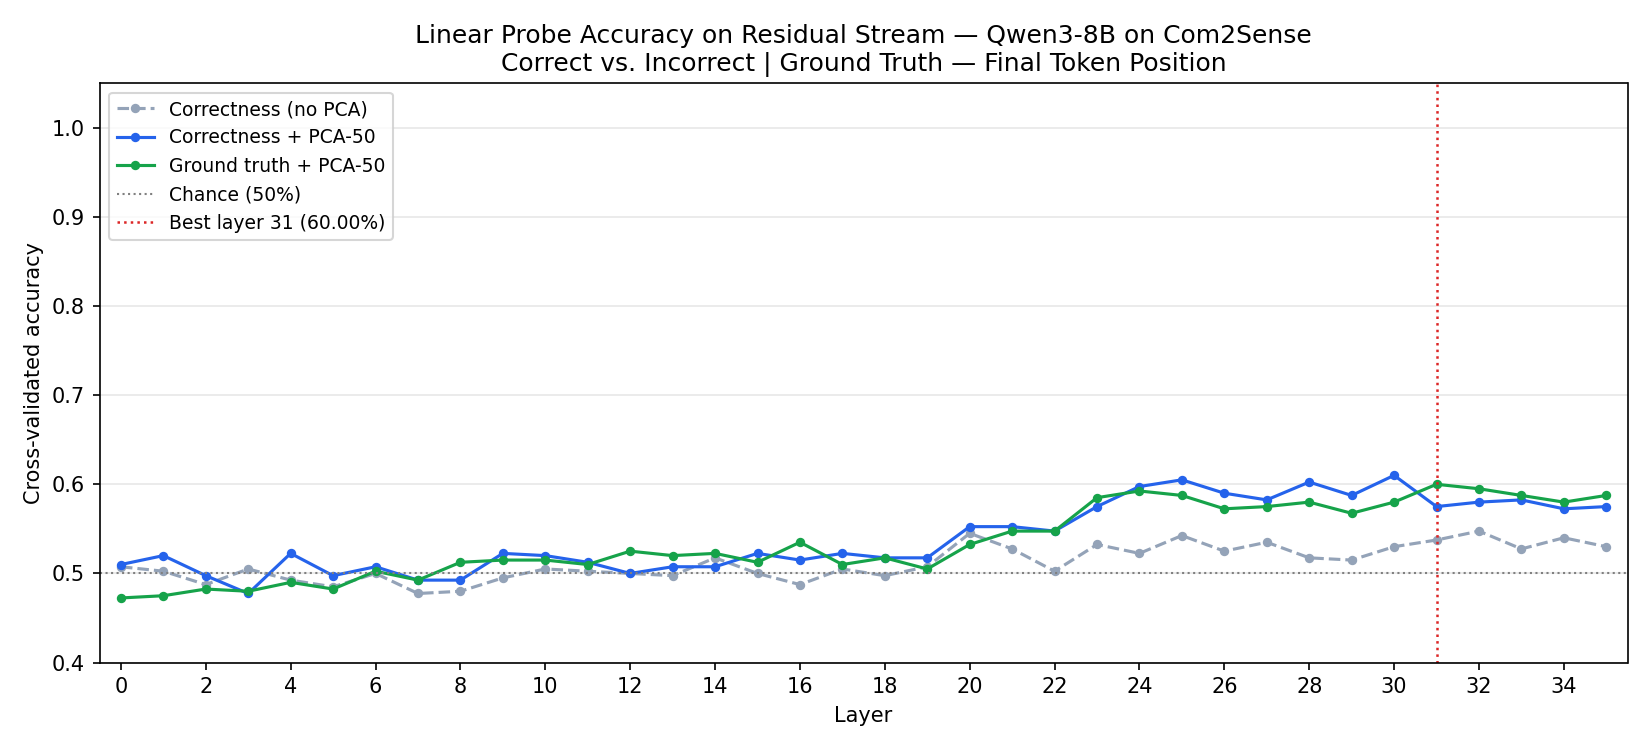
\includegraphics[width=0.48\linewidth]{reports/figures/probe_accuracy_curve.png}
\hfill
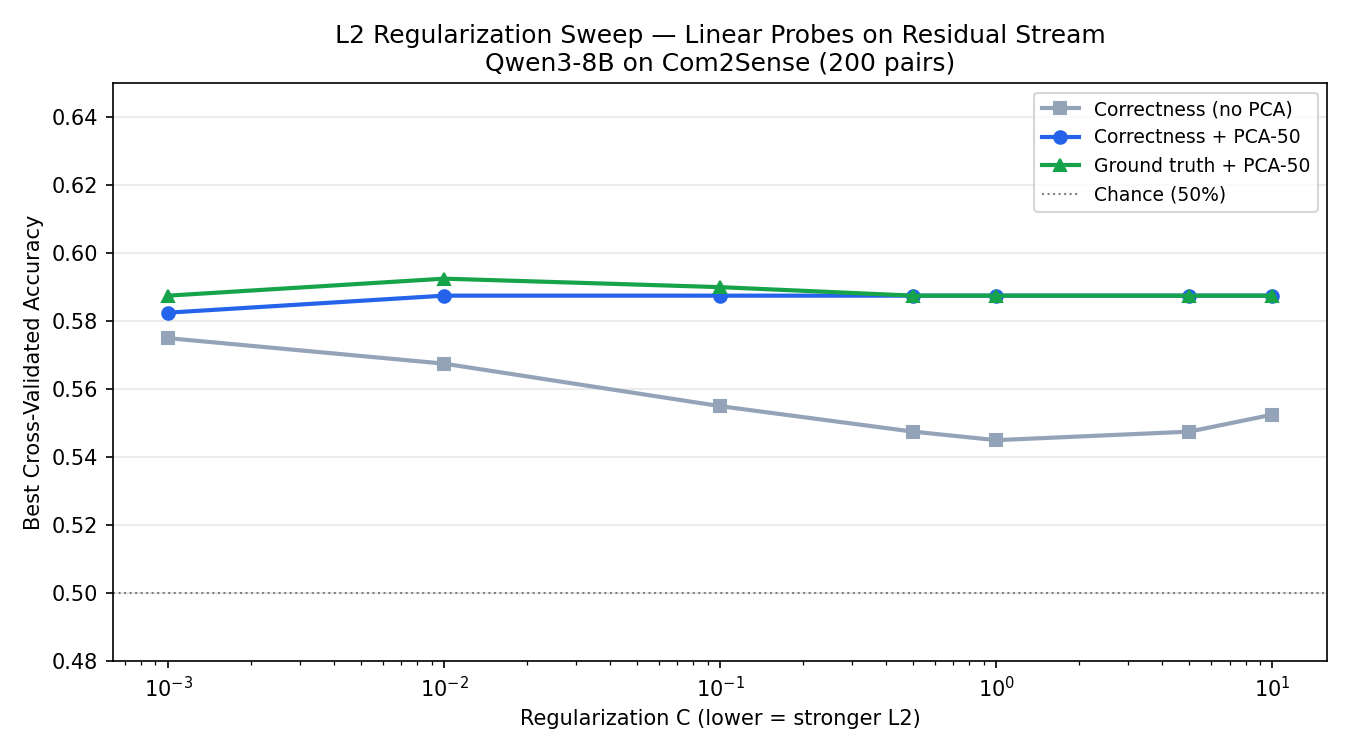
\includegraphics[width=0.48\linewidth]{reports/figures/l2_sweep_results.png}
\caption{\textbf{Left:} Per-layer probing accuracy for three probe configurations. Signal is at chance through layers 0--19 and rises from layer~20. \textbf{Right:} $L_2$ regularization sweep. The corrected probing ceiling is ${\sim}59$\%.}
\label{fig:probing}
\end{figure}

\subsection{Phase 3: Activation patching}

\paragraph{Layer-level patching.}
Figure~\ref{fig:patching} shows the results of replacing the incorrect example's full residual stream with the correct example's at each layer.
Across all 18 layers (18--35), the \textbf{prediction flip rate is 0\%}---no single layer's activation is sufficient to repair the prediction.
All logit changes are negative, ranging from $-0.006$ (L18) to $-0.355$ (L35), meaning patching consistently \emph{degrades} predictions.
This monotonic degradation reflects distributional mismatch: the correct and incorrect examples are different sentences, and replacing the entire post-layer state creates activations that are inconsistent with what downstream layers expect.

\begin{figure}[t]
\centering
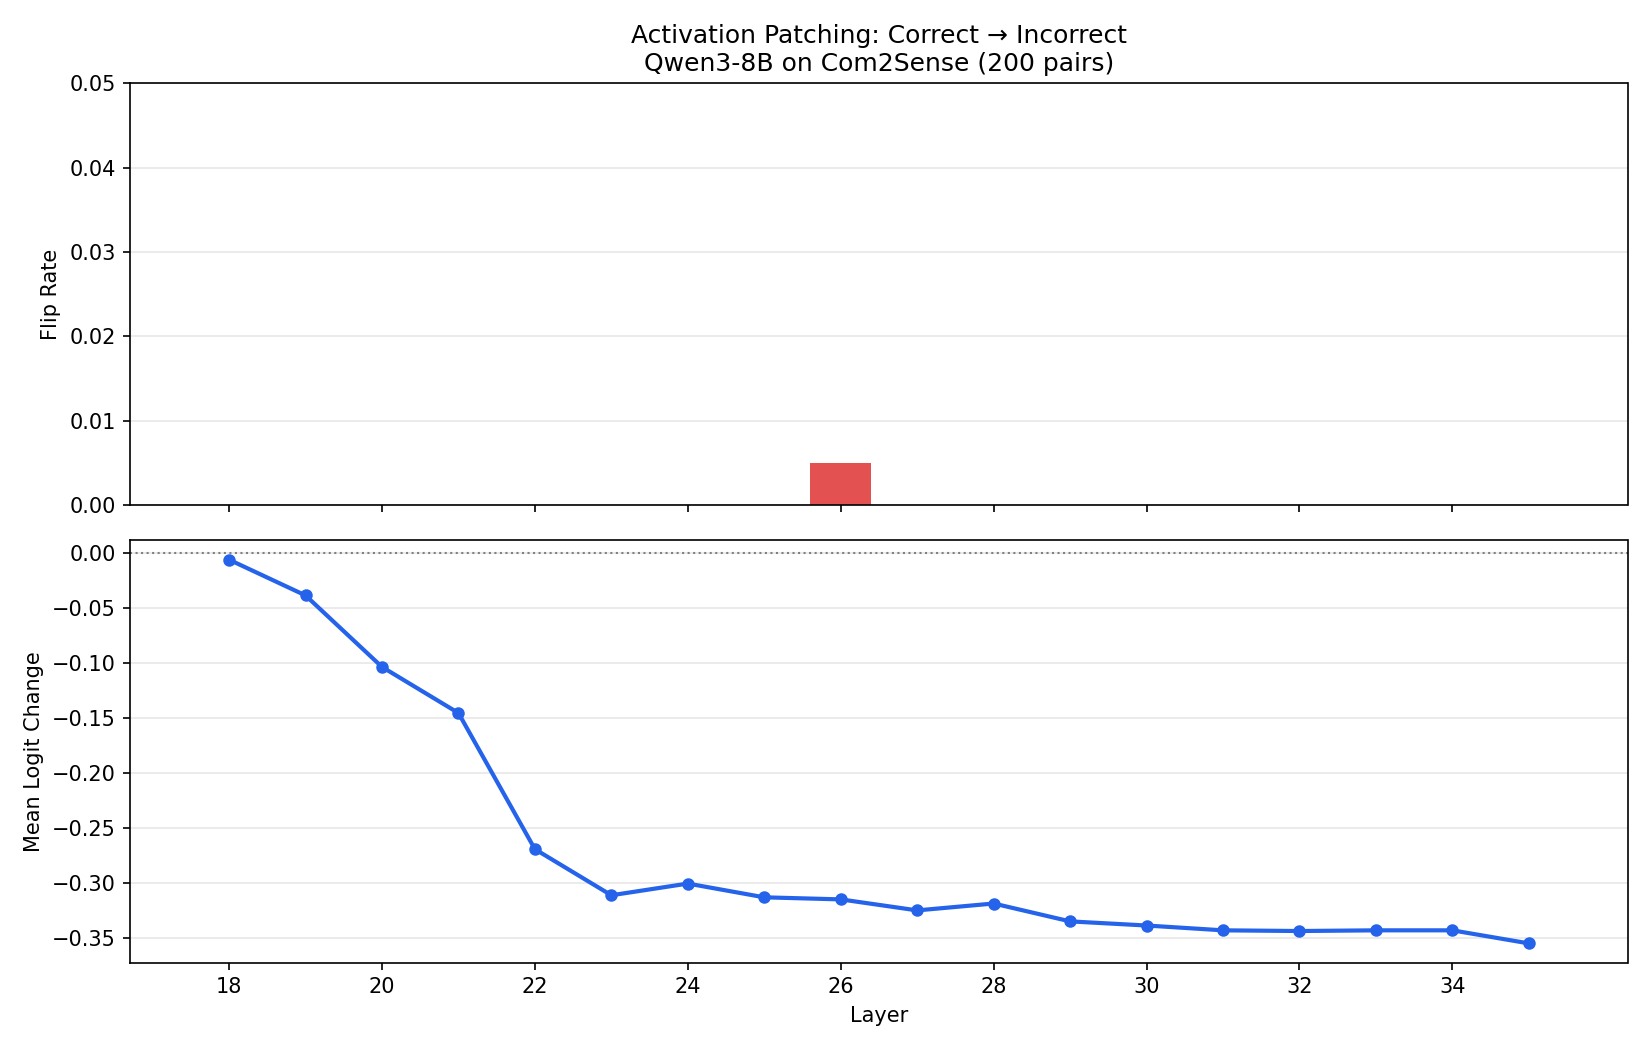
\includegraphics[width=\linewidth]{reports/figures/patching_results.png}
\caption{Layer-level activation patching results (layers 18--35). Flip rate is 0\% at all layers; logit change is uniformly negative and grows in magnitude with depth, reflecting distributional mismatch from full-stream replacement.}
\label{fig:patching}
\end{figure}

\paragraph{Head-level patching.}
Figure~\ref{fig:head_analysis} (left) shows the top~10 attention heads by mean absolute patching effect.
The most influential head (L20.H8) moves the logit by 0.147 on average---negligible compared to the mean correct--incorrect logit gap of 2.534.
No head produces any prediction flips.

\paragraph{Head-level probing.}
Figure~\ref{fig:head_analysis} (right) shows the layer $\times$ head probing accuracy heatmap.
The best individual head (L32.H20) achieves 59.50\%---nearly identical to the full residual-stream probe (${\sim}59$\%).
No head stands out; the signal is weakly but redundantly present across many heads.
Crucially, \textbf{the most informative heads differ from the most causally influential heads}: the probing leaders (L32, L34) are distinct from the patching leaders (L20, L21), demonstrating that information presence and causal influence are dissociated.

\begin{figure}[t]
\centering
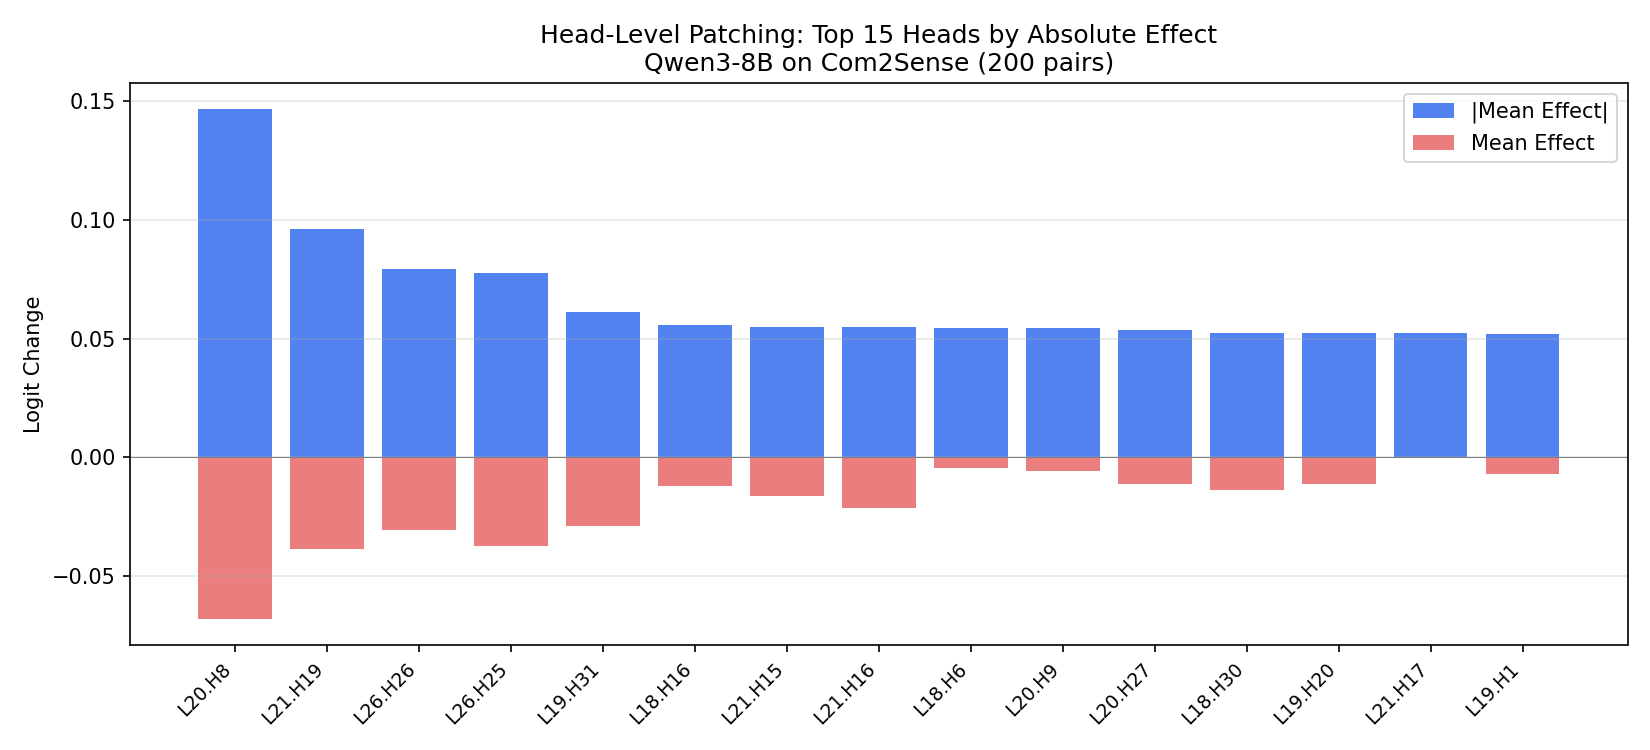
\includegraphics[width=0.48\linewidth]{reports/figures/head_patching_results.png}
\hfill
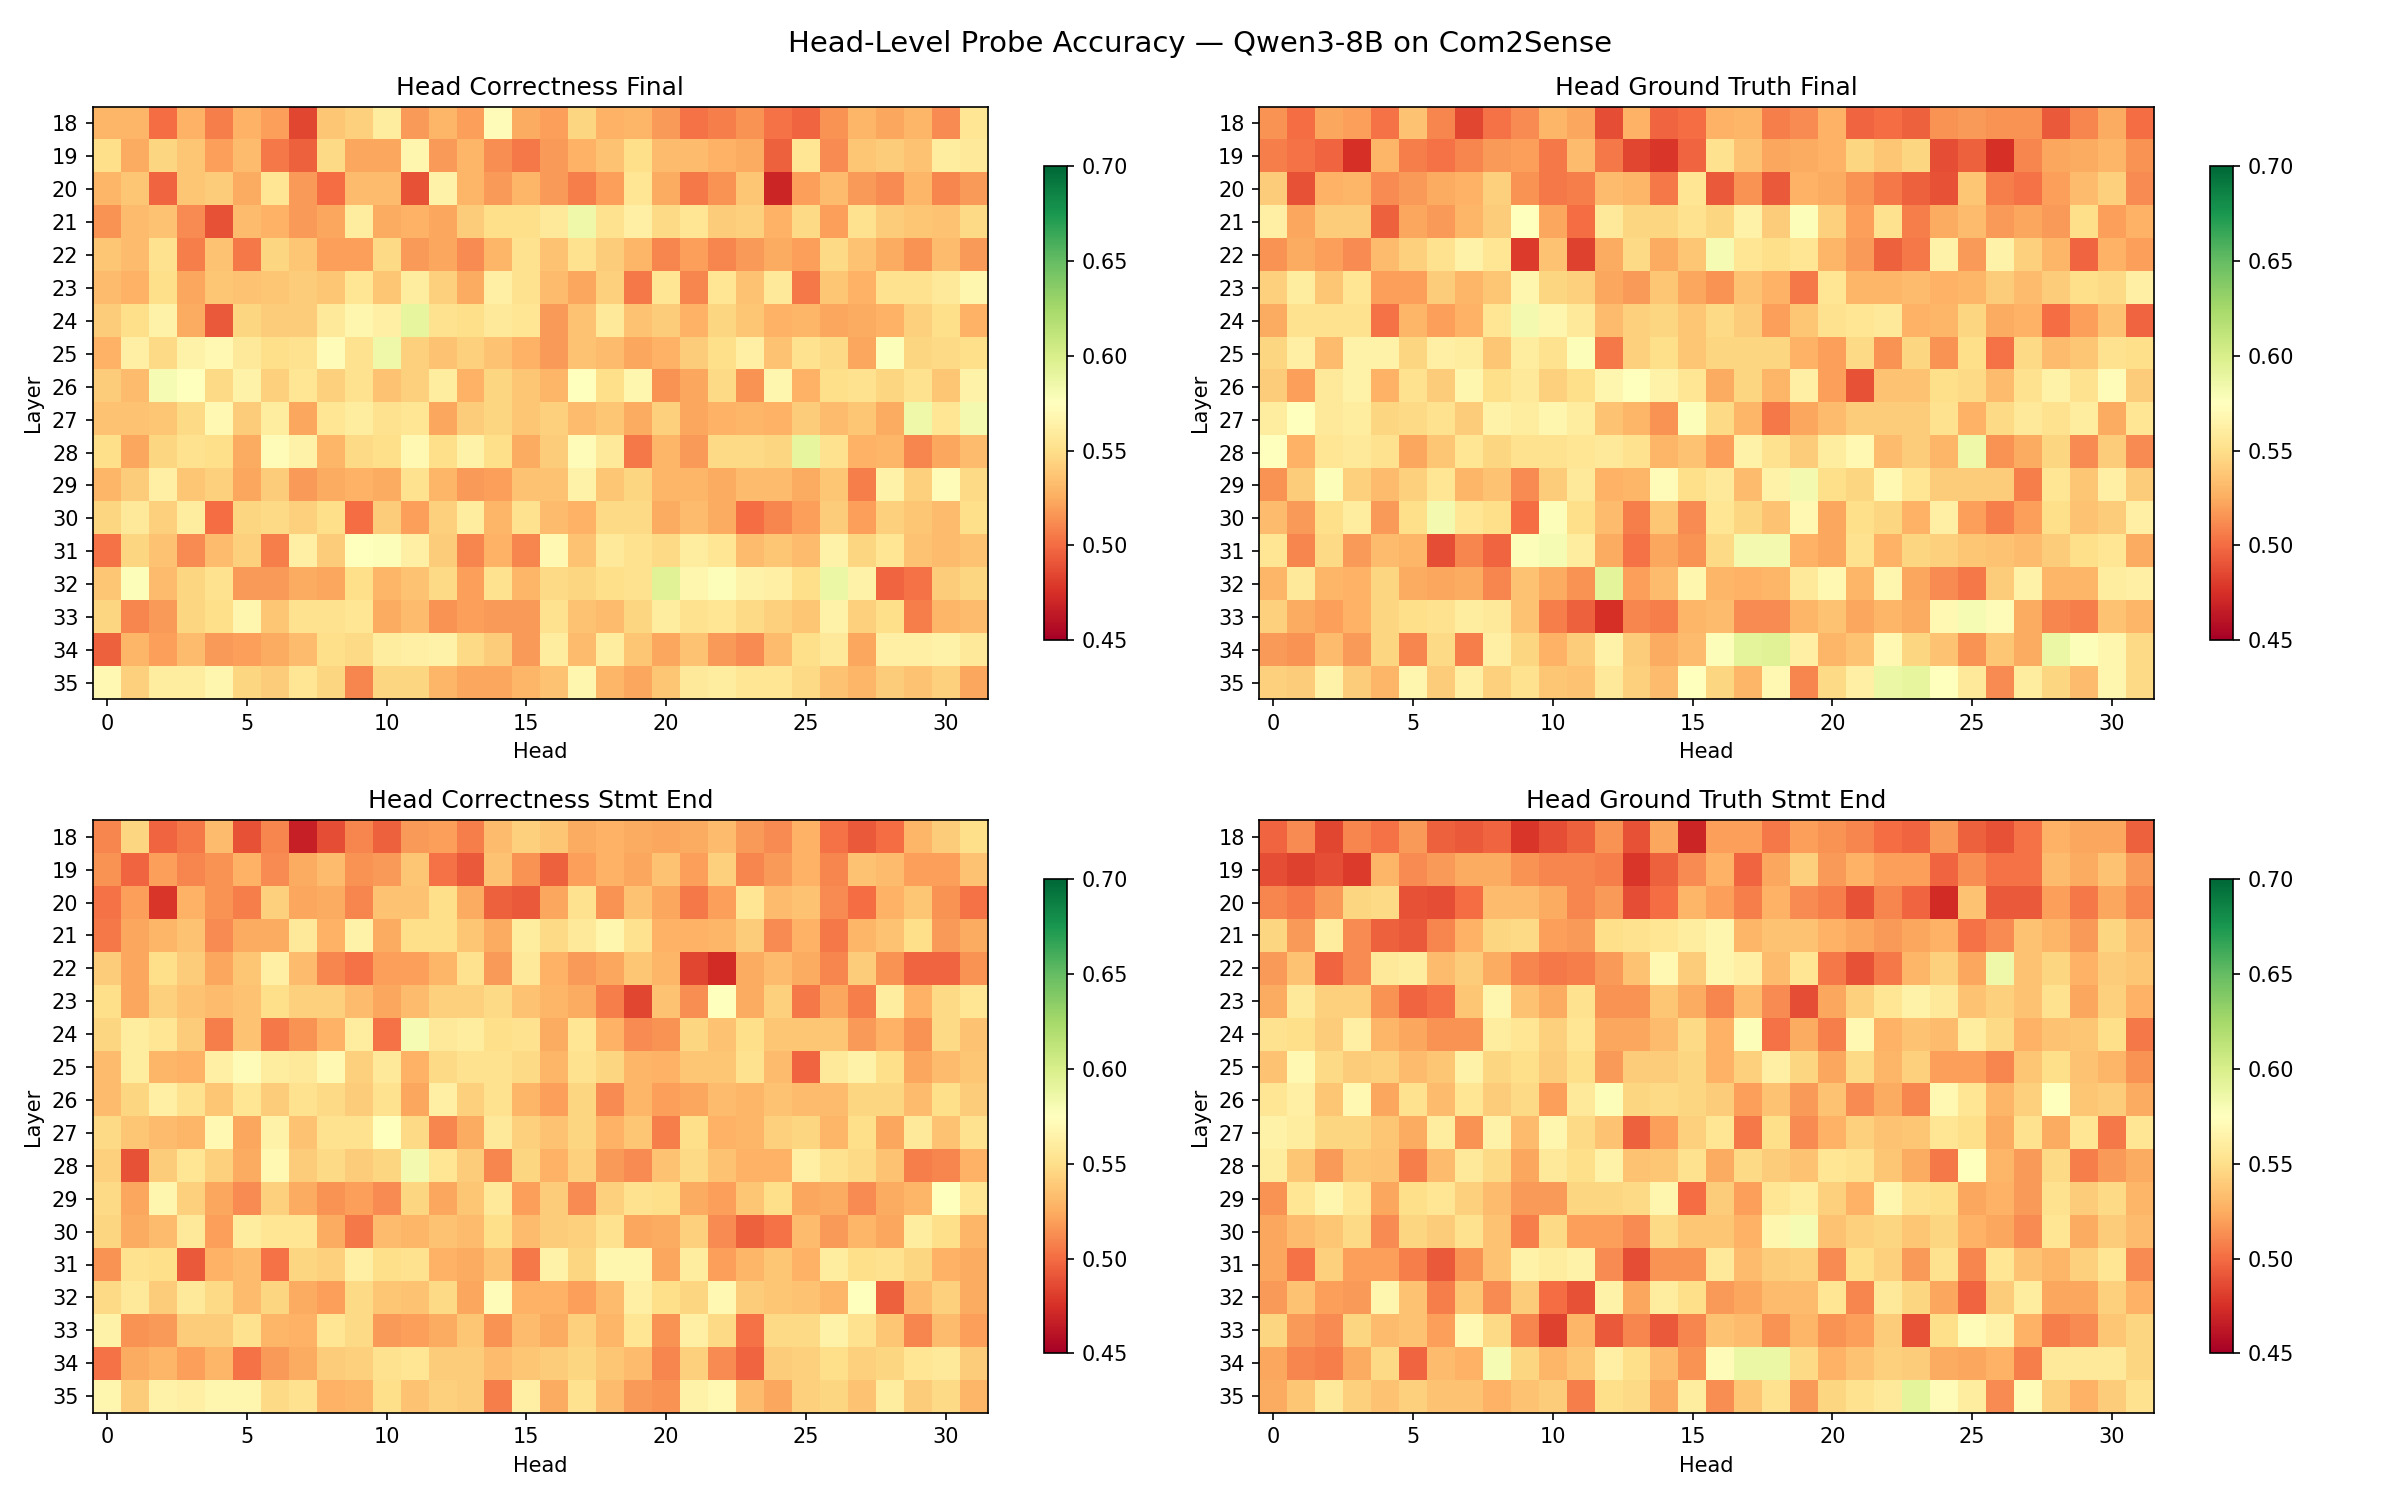
\includegraphics[width=0.48\linewidth]{reports/figures/head_probe_heatmap.png}
\caption{\textbf{Left:} Top attention heads by mean absolute patching effect. Maximum effect is 0.147 (L20.H8); no head produces prediction flips. \textbf{Right:} Layer $\times$ head probing accuracy heatmap. Best individual head (59.5\%) matches full-stream accuracy, indicating the signal is redundantly distributed.}
\label{fig:head_analysis}
\end{figure}

\paragraph{Mean-ablation.}
Table~\ref{tab:ablation} shows the results of mean-ablating each of the 17 candidate heads on the 200 correct examples.
The maximum flip rate is \textbf{1.0\%} (L26.H25, 2 flips out of 200), and the maximum absolute logit change is 0.028 (L18.H6)---negligible.
No head is necessary for correct commonsense predictions (selected results shown; see Appendix~\ref{app:ablation} for all 17 heads).
This result complements the patching findings: patching tests sufficiency (no component is sufficient), while ablation tests necessity (no component is necessary).
Together, they establish that commonsense reasoning is genuinely distributed.

\begin{table}[t]
\centering
\small
\caption{Mean-ablation results for the 17 candidate heads (sorted by flip count). Source indicates whether the head was identified by patching or probing.}
\label{tab:ablation}
\begin{tabular}{lrrrrl}
\toprule
\textbf{Head} & \textbf{Flips} & \textbf{Flip\%} & \textbf{Mean $\Delta$logit} & \textbf{Std} & \textbf{Source} \\
\midrule
L26.H25 & 2 & 1.0\% & $+0.007$ & 0.153 & Patching \\
L20.H8  & 1 & 0.5\% & $+0.003$ & 0.186 & Patching \\
L21.H19 & 1 & 0.5\% & $-0.014$ & 0.126 & Patching \\
L26.H26 & 1 & 0.5\% & $+0.014$ & 0.156 & Patching \\
L19.H31 & 1 & 0.5\% & $-0.006$ & 0.096 & Patching \\
L21.H16 & 1 & 0.5\% & $-0.001$ & 0.084 & Patching \\
L28.H25 & 1 & 0.5\% & $-0.004$ & 0.073 & Probing \\
\midrule
L18.H6  & 0 & 0.0\% & $+0.028$ & 0.081 & Patching \\
L32.H20 & 0 & 0.0\% & $+0.003$ & 0.067 & Probing \\
L34.H18 & 0 & 0.0\% & $+0.002$ & 0.069 & Probing \\
L35.H23 & 0 & 0.0\% & $-0.006$ & 0.073 & Probing \\
\bottomrule
\end{tabular}
\end{table}

\subsection{Phase 4: Logit-lens trajectory analysis}

The logit-lens analysis fundamentally refines our understanding of failure timing.
Figure~\ref{fig:logit_lens} (left) shows the aggregate signed logit gap trajectories for correct and incorrect examples across all 36 layers.
The trajectories reveal a striking three-stage pattern:

\begin{enumerate}
    \item \textbf{Early divergence (layers 0--4):} Correct and incorrect trajectories start separated from layer~0 ($+0.97$ vs.\ $-0.97$), already pointing in opposite directions.
    \item \textbf{Mid-layer convergence (layers 5--19):} Both trajectories partially reverse toward zero, with correct examples briefly turning negative at layers 10--15 and incorrect examples briefly turning positive.
    \item \textbf{Late amplification (layers 20--35):} Trajectories re-diverge sharply from layer~20, peaking at $\pm 11$ around layer~30 before settling to $\pm 2.5$ at the final layer.
\end{enumerate}

\paragraph{Failure timing.}
Among the 200 incorrect examples, \textbf{76.5\% (153/200) are already directionally wrong at layer~0}---the signed gap is negative from the first measured layer.
Table~\ref{tab:logit_lens} shows that the mean first-wrong layer is 1.61, but the mean \emph{stable}-wrong layer (where the wrong-answer bias becomes sustained) is 19.9---matching the layer range where probing first detects signal.
This two-stage pattern---early bias followed by late consolidation---is more nuanced than either a pure retrieval failure or a pure inference failure.

\begin{table}[t]
\centering
\small
\caption{Logit-lens failure timing statistics (200 incorrect examples).}
\label{tab:logit_lens}
\begin{tabular}{lc}
\toprule
\textbf{Metric} & \textbf{Value} \\
\midrule
Wrong at layer 0 & 76.5\% (153/200) \\
Mean first-wrong layer & 1.61 \\
Mean stable-wrong layer & 19.9 \\
Mean stable-correct layer (correct examples) & 20.2 \\
Mean final gap (correct examples) & $+2.81$ \\
Mean final gap (incorrect examples) & $-2.53$ \\
\midrule
\multicolumn{2}{l}{\textit{Final gap by domain (incorrect examples):}} \\
Social & $-3.52$ \\
Temporal & $-2.30$ \\
Time & $-2.20$ \\
\bottomrule
\end{tabular}
\end{table}

\begin{figure}[t]
\centering
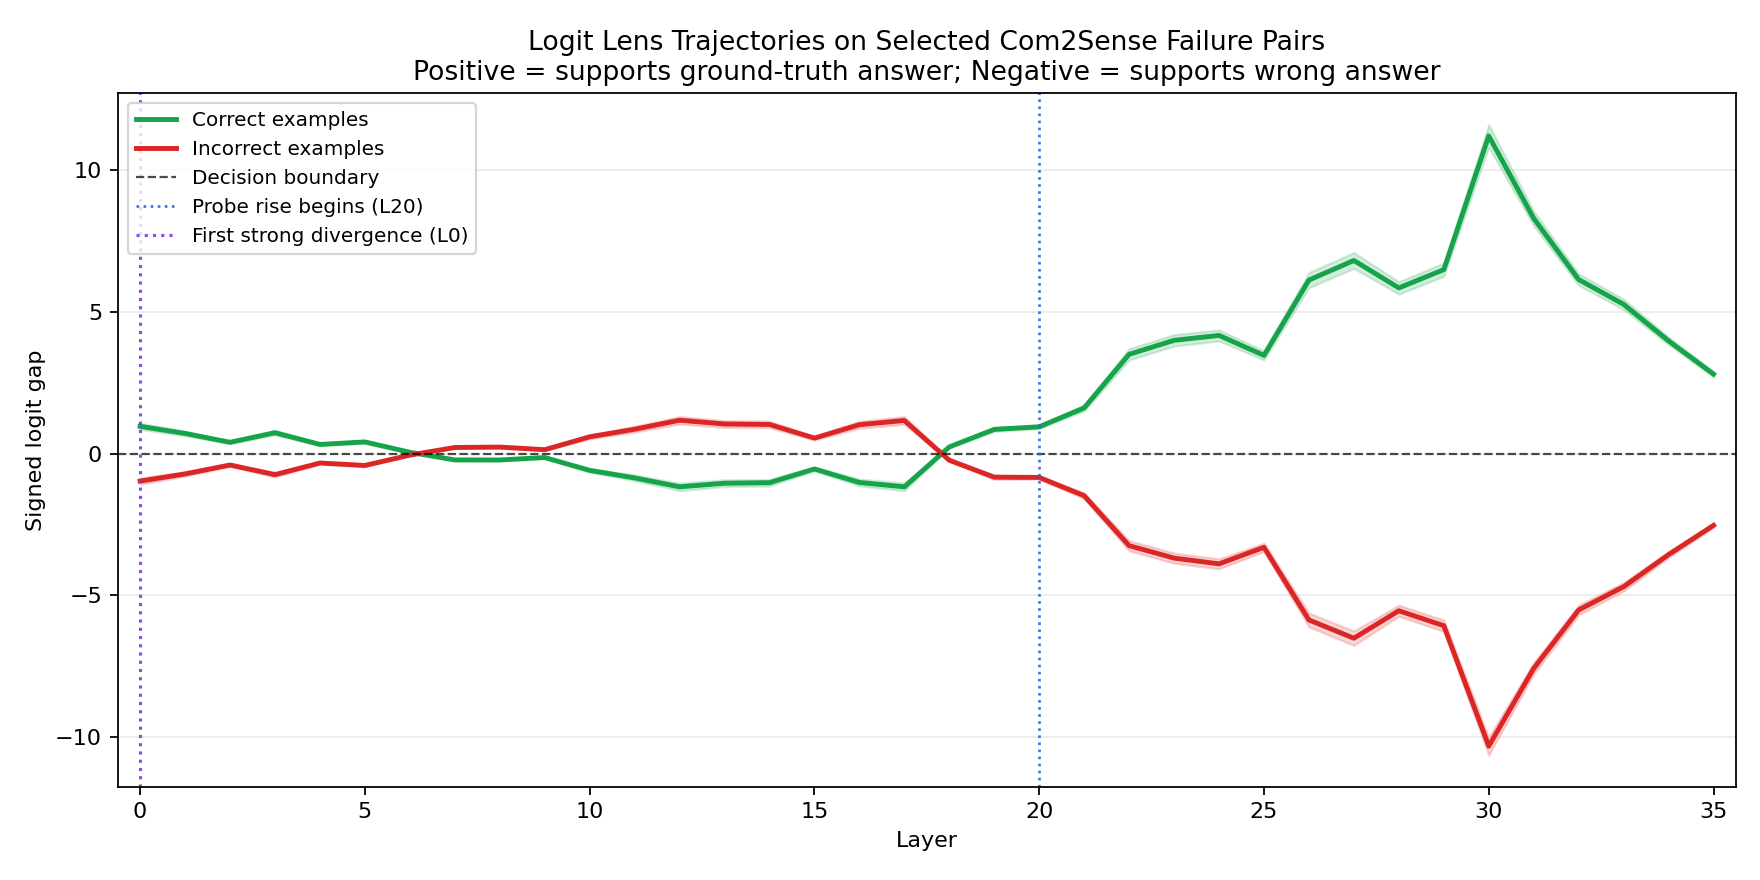
\includegraphics[width=0.55\linewidth]{reports/figures/logit_lens_trajectories.png}
\hfill
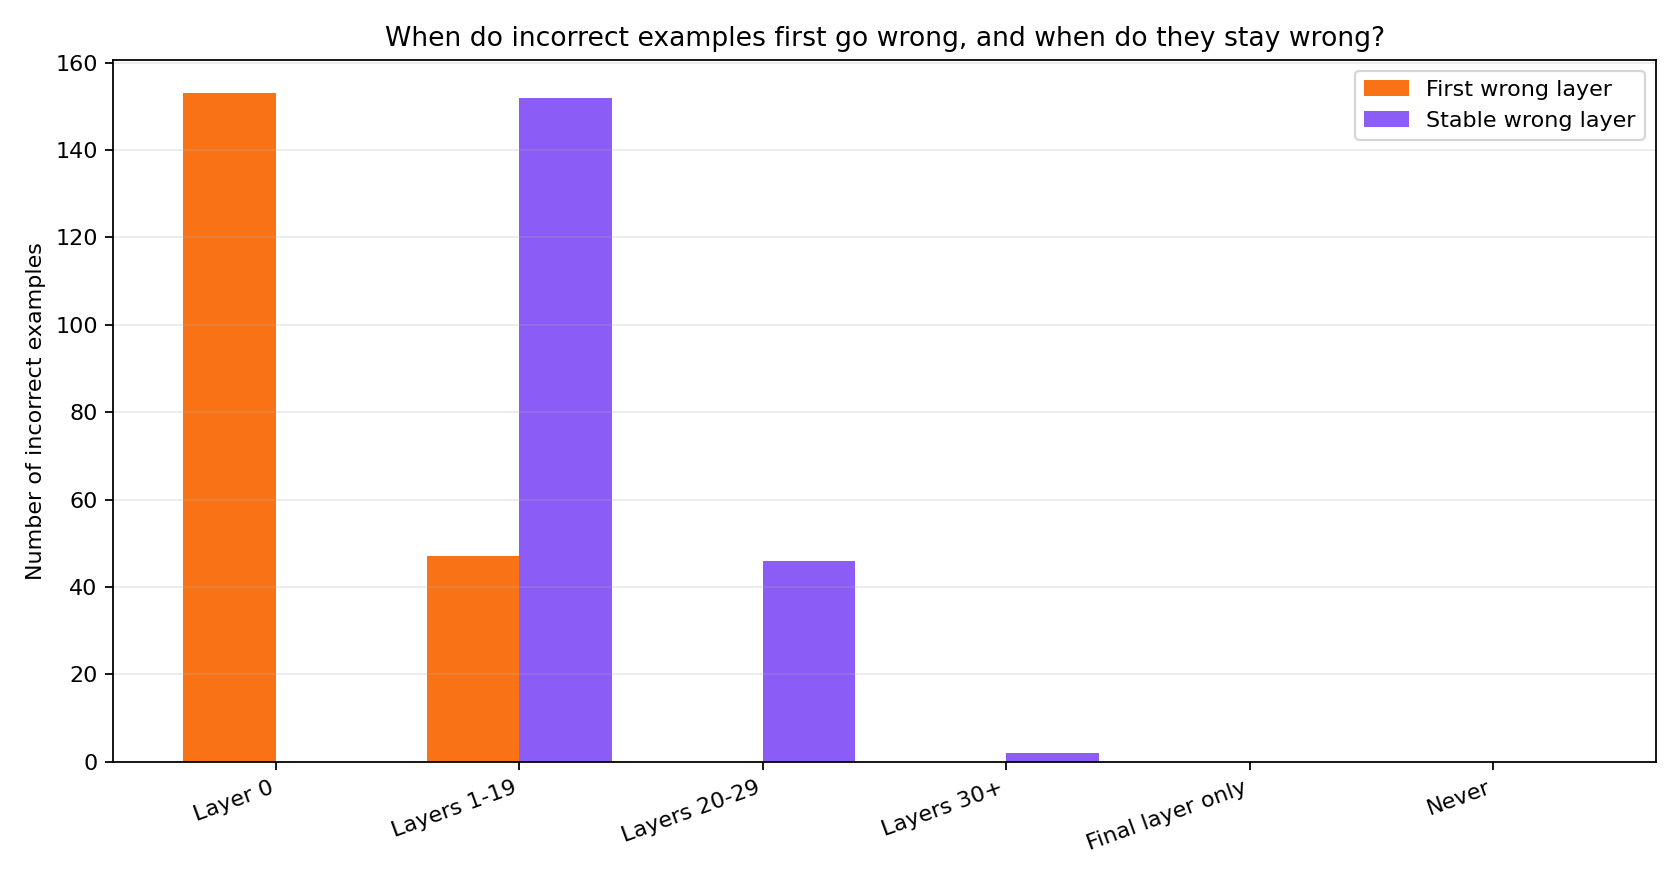
\includegraphics[width=0.42\linewidth]{reports/figures/logit_lens_failure_layers.png}
\caption{\textbf{Left:} Aggregate logit-lens trajectories. Signed logit gap (positive = supports ground truth) for correct (green) and incorrect (red) examples across 36 layers. Trajectories diverge at layer~0, partially converge through mid-layers, then re-diverge strongly from layer~20. \textbf{Right:} Distribution of first-wrong (orange) and stable-wrong (blue) layers for the 200 incorrect examples.}
\label{fig:logit_lens}
\end{figure}

\paragraph{Domain-level trajectories.}
Figure~\ref{fig:domain_trajectories} shows logit-lens trajectories broken down by domain for incorrect examples.
Social failures end in the strongest wrong-state ($-3.52$), consistent with the highest false-bias rate (77.9\%).
Temporal failures show the weakest final wrong-state ($-2.30$) but the lowest behavioral accuracy (63.53\%), suggesting that temporal failures are more evenly distributed between confident wrong answers and uncertain wrong answers.

\subsection{Phase 5: MLP vs.\ attention sublayer decomposition}

To test whether commonsense signal concentrates in attention or MLP sublayers---as a concurrent class project found MLP dominance for physical-commonsense tasks on PIQA~\citep{bisk2020piqa} using GPT-2 Small---we decompose layer patching into separate \texttt{hook\_attn\_out} and \texttt{hook\_mlp\_out} interventions.

Table~\ref{tab:sublayer} shows selected results.
Unlike full \texttt{resid\_post} patching (uniformly negative), sublayer patching shows \emph{mixed signs}---some layers produce positive logit changes, others negative.
This sign variability reveals that the monotonically negative \texttt{resid\_post} results were an artifact of compounding distributional mismatch, not evidence of layer-specific causal importance.

\paragraph{Neither sublayer dominates.}
The only prediction flips occur at L25~attention (1.5\% flip rate, $+0.163$ mean logit change---the largest positive intervention in the entire study) and L35~MLP (1.5\% flip rate, $+0.133$).
Attention effects are larger in magnitude in middle layers (L19--L27), while MLP effects match or exceed attention only at L22--L23 and in late layers (L30--L35).
This differs from the MLP-dominance pattern found in the concurrent GPT-2 Small / PIQA study, likely reflecting both architectural differences (Qwen3-8B uses grouped-query attention) and task differences (Com2Sense requires multi-hop causal/temporal reasoning vs.\ PIQA's single-step physical intuition).

\begin{table}[t]
\centering
\small
\caption{Selected MLP vs.\ attention sublayer patching results (layers 18--35).}
\label{tab:sublayer}
\begin{tabular}{lrrrr}
\toprule
\textbf{Layer} & \textbf{Attn flip\%} & \textbf{Attn $\Delta$logit} & \textbf{MLP flip\%} & \textbf{MLP $\Delta$logit} \\
\midrule
18 & 0.0\% & $-0.011$ & 0.0\% & $-0.003$ \\
20 & 0.0\% & $-0.081$ & 0.0\% & $-0.014$ \\
22 & 0.0\% & $-0.156$ & 0.0\% & $-0.149$ \\
\textbf{25} & \textbf{1.5\%} & $\mathbf{+0.163}$ & 0.0\% & $+0.007$ \\
28 & 0.0\% & $+0.003$ & 0.0\% & $-0.045$ \\
32 & 0.0\% & $-0.011$ & 0.0\% & $-0.012$ \\
\textbf{35} & 0.0\% & $-0.018$ & \textbf{1.5\%} & $\mathbf{+0.133}$ \\
\bottomrule
\end{tabular}
\end{table}

%=============================================================================
\section{Discussion}
\label{sec:discussion}
%=============================================================================

\subsection{Answers to research questions}

\paragraph{Q1: Localized or distributed?}
\textbf{Distributed.} The convergent evidence across all experiments is unambiguous:
\begin{itemize}
    \item Layer-level patching: 0\% flip rate across 18 layers (no layer is sufficient).
    \item Head-level patching: 0\% flip rate across 160 combinations (no head is sufficient).
    \item Sublayer patching: maximum 1.5\% flip rate (neither attention nor MLP is sufficient).
    \item Mean-ablation: maximum 1.0\% flip rate across 17 candidate heads (no head is necessary).
    \item Head-level probing: best head (59.5\%) matches full-stream accuracy (${\sim}59$\%), indicating the signal is redundantly spread rather than concentrated.
\end{itemize}
This contrasts sharply with factual recall findings.
\citet{geva2023dissecting} report flip rates of 30--60\%+ for factual associations.
\citet{wang2022interpretability} identify a specific circuit for indirect object identification.
Commonsense reasoning---with its demand for multi-hop world knowledge integration---does not admit such localization.

\paragraph{Q2: Knowledge retrieval or inference failure?}
\textbf{Early bias with late consolidation.}
The probing results initially suggested a purely late-onset inference failure (signal emerging at layer~20, chance before that).
Logit-lens analysis reveals a more nuanced two-stage process:
76.5\% of incorrect examples are already directionally wrong at layer~0, suggesting an \emph{early representational bias}---possibly reflecting training data priors such as the observed false-bias (the model defaults to rejection under uncertainty).
However, these early biases are not stably committed until ${\sim}$layer~20, and the non-monotonic trajectory (with mid-layer reversals) shows the network iteratively revises its judgment before final consolidation.

This is inconsistent with either a pure retrieval failure (the model never had the knowledge) or a pure inference failure (wrong computation on correct representations).
Instead, the model builds an early weak bias toward the wrong answer, then consolidates it through late-layer computation.

\paragraph{Q3: Architectural, representational, or training-induced?}
\textbf{Representational, with possible training-data contributions.}
The evidence most strongly supports a representational deficit:
\begin{itemize}
    \item Probing accuracy of ${\sim}59$\% means the residual stream carries only weak signal about commonsense truth. The model never builds a strong enough internal representation to reliably distinguish correct from incorrect reasoning.
    \item The architecture \emph{can} encode commonsense distinctions ($59$\% $> 50$\%), just weakly. A purely architectural limitation would more likely show 50\% (no signal at all) or concentrate signal in specific components.
    \item The sublayer decomposition shows that attention can transiently encode useful signal (L25 attention: $+0.163$), but not consistently enough for reliable judgment. The architecture is not the bottleneck; the \emph{strength} of the representation is.
\end{itemize}
We cannot fully distinguish representational from training-induced with our methods.
If the model never encountered sufficient commonsense reasoning examples during training, the representational deficit would be a consequence of training data limitations.
Distinguishing these would require comparing models trained on different data mixtures, which is beyond our scope.

\subsection{Comparison with prior work}

Table~\ref{tab:comparison} places our findings in the context of prior mechanistic studies.
The near-zero flip rates we observe are dramatically lower than those reported for factual tasks, establishing that commonsense reasoning is mechanistically distinct from factual recall.

\begin{table}[t]
\centering
\small
\caption{Comparison with prior mechanistic interpretability studies.}
\label{tab:comparison}
\begin{tabular}{llll}
\toprule
\textbf{Study} & \textbf{Task} & \textbf{Method} & \textbf{Flip rate} \\
\midrule
\citet{wang2022interpretability} & IOI (GPT-2) & Circuit patching & $>$70\% \\
\citet{geva2023dissecting} & Factual recall & Layer patching & 30--60\%+ \\
\citet{meng2022locating} & Factual editing & ROME (MLP) & $>$95\% \\
\textbf{This work} & Commonsense & Layer patching & \textbf{0\%} \\
\textbf{This work} & Commonsense & Head patching & \textbf{0\%} \\
\textbf{This work} & Commonsense & Sublayer patching & \textbf{1.5\%} \\
\textbf{This work} & Commonsense & Mean-ablation & \textbf{1.0\%} \\
\bottomrule
\end{tabular}
\end{table}

\subsection{Limitations}

This study is limited to a single model (Qwen3-8B) and a single dataset (Com2Sense).
The 200-pair subset, while sufficient for reliable statistical patterns, may not capture all failure modes.
Probing accuracy of ${\sim}59$\% is real but weak; stronger probes (e.g., nonlinear probes, token-averaged representations) might reveal more structure.
We do not ablate full attention layers or MLP blocks, only individual heads; block-level ablation might reveal stronger effects.
Causal attribution from activation patching is limited by distributional mismatch between different input sentences; path patching~\citep{conmy2023towards}, which controls for this mismatch, could reveal additional structure.
Finally, we cannot fully distinguish representational from training-induced failures without comparing models trained on different data mixtures.

%=============================================================================
\section{Conclusion}
\label{sec:conclusion}
%=============================================================================

We have presented a systematic mechanistic interpretability study of commonsense reasoning failures in Qwen3-8B, combining five complementary techniques across 200 asymmetric complementary pairs from Com2Sense.
Our central finding is that commonsense failures are \emph{fundamentally distributed}: no single layer, attention head, or sublayer is sufficient (0--1.5\% flip rates) or necessary (maximum 1\% flip rate under ablation) for correct commonsense predictions.

Logit-lens analysis reveals that failures involve an \emph{early-bias, late-consolidation} process: 76.5\% of incorrect predictions are already directionally wrong at layer~0, but the wrong answer typically stabilizes around layer~20.
Probing accuracy plateaus at ${\sim}59$\%, indicating weak but genuine signal that is redundantly spread across the residual stream rather than concentrated in identifiable components.

These findings challenge the assumption that commonsense failures can be diagnosed and repaired through the same localized circuit-finding methodology that has proven successful for factual recall.
Commonsense reasoning appears to require a fundamentally different treatment: strengthening the underlying representational encoding through training, rather than patching specific computational components after the fact.
The stark contrast with prior localized findings likely reflects both architectural differences (Qwen3-8B's 36-layer grouped-query attention architecture vs.\ GPT-2 Small's 12-layer model) and dataset differences (Com2Sense's multi-hop causal and temporal judgments vs.\ single-fact retrieval tasks), suggesting that the degree of circuit localization depends heavily on the complexity of the reasoning required.

\section*{Acknowledgments}
We thank our advisor Darin Keng for guidance throughout this project.
We also thank the TransformerLens team~\citep{nanda2022transformerlens} for their interpretability toolkit and Modal~\citep{modal2023} for providing GPU compute infrastructure.
All experiments were conducted on A100-80GB GPUs.

\bibliography{paper}
\bibliographystyle{colm2026_conference}

%=============================================================================
\appendix
%=============================================================================

\section{Additional figures}
\label{app:figures}

\begin{figure}[h]
\centering
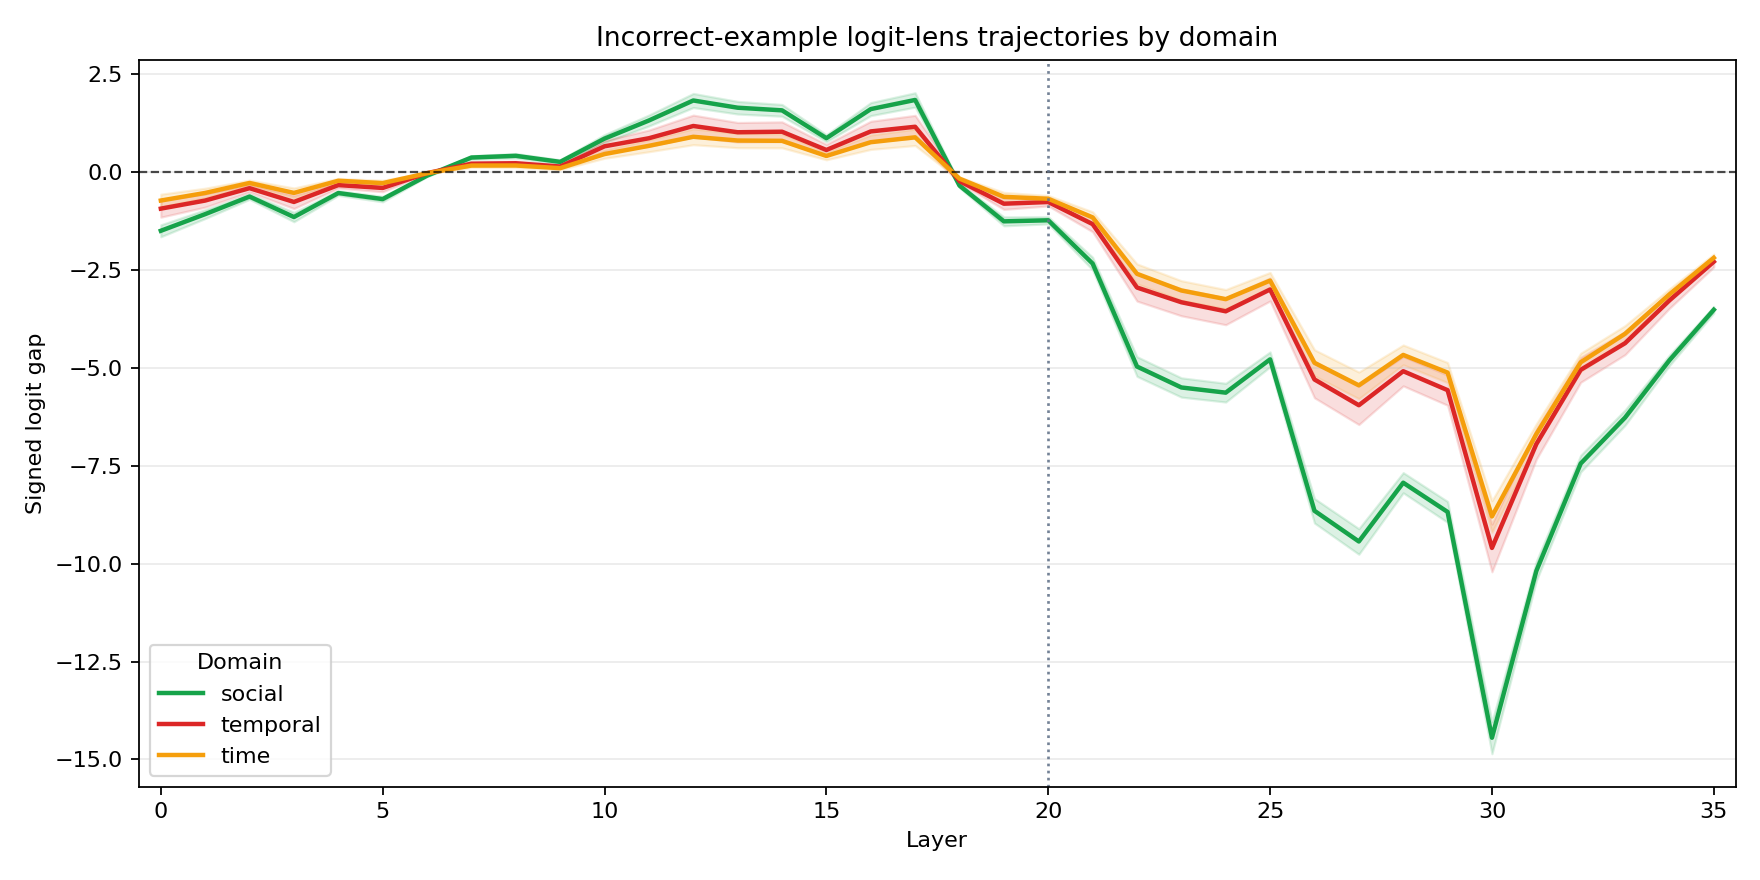
\includegraphics[width=\linewidth]{reports/figures/logit_lens_domain_trajectories.png}
\caption{Logit-lens trajectories broken down by domain for incorrect examples. Social failures show the most extreme final wrong-state ($-3.52$), while temporal failures show the weakest ($-2.30$).}
\label{fig:domain_trajectories}
\end{figure}

\begin{figure}[h]
\centering
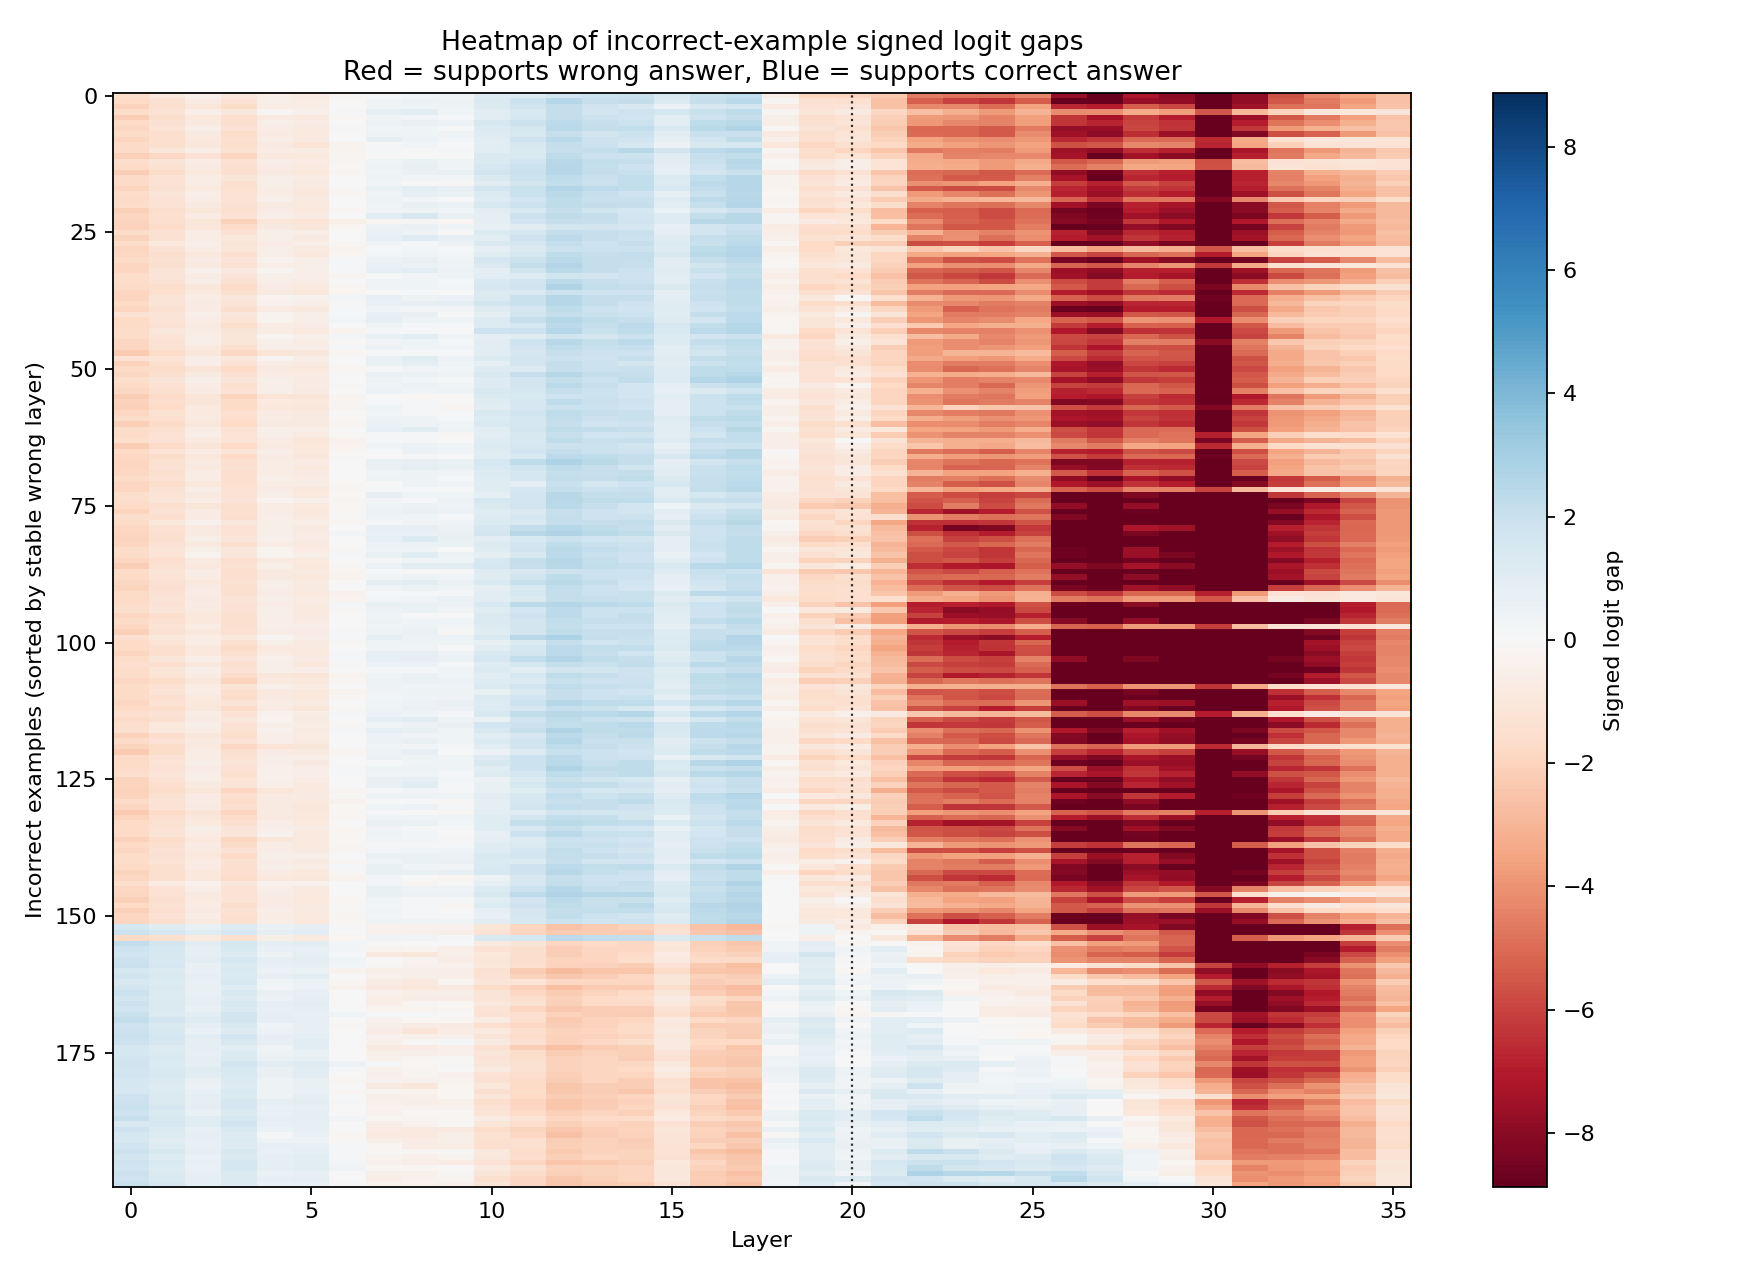
\includegraphics[width=\linewidth]{reports/figures/logit_lens_incorrect_heatmap.png}
\caption{Heatmap of signed logit gaps for all 200 incorrect examples across 36 layers. Rows are individual examples, columns are layers. Most examples are red (wrong direction) from early layers; a minority start blue (correct direction) and transition to red around layer~20.}
\label{fig:heatmap}
\end{figure}

\section{Full sublayer patching results}
\label{app:sublayer}

\begin{table}[h]
\centering
\small
\caption{Complete MLP vs.\ attention sublayer patching results for all 18 layers (18--35).}
\label{tab:full_sublayer}
\begin{tabular}{lrrrr}
\toprule
\textbf{Layer} & \textbf{Attn flip\%} & \textbf{Attn $\Delta$logit} & \textbf{MLP flip\%} & \textbf{MLP $\Delta$logit} \\
\midrule
18 & 0.0\% & $-0.011$ & 0.0\% & $-0.003$ \\
19 & 0.0\% & $-0.037$ & 0.0\% & $-0.011$ \\
20 & 0.0\% & $-0.081$ & 0.0\% & $-0.014$ \\
21 & 0.0\% & $-0.063$ & 0.0\% & $+0.009$ \\
22 & 0.0\% & $-0.156$ & 0.0\% & $-0.149$ \\
23 & 0.0\% & $-0.061$ & 0.0\% & $-0.146$ \\
24 & 0.0\% & $-0.041$ & 0.0\% & $+0.077$ \\
25 & 1.5\% & $+0.163$ & 0.0\% & $+0.007$ \\
26 & 0.0\% & $-0.090$ & 0.0\% & $-0.072$ \\
27 & 0.0\% & $-0.060$ & 0.0\% & $-0.051$ \\
28 & 0.0\% & $+0.003$ & 0.0\% & $-0.045$ \\
29 & 0.0\% & $-0.055$ & 0.0\% & $-0.051$ \\
30 & 0.0\% & $-0.066$ & 0.0\% & $-0.083$ \\
31 & 0.0\% & $-0.019$ & 0.0\% & $+0.023$ \\
32 & 0.0\% & $-0.011$ & 0.0\% & $-0.012$ \\
33 & 0.0\% & $-0.032$ & 0.0\% & $-0.002$ \\
34 & 0.0\% & $-0.030$ & 0.0\% & $-0.016$ \\
35 & 0.0\% & $-0.018$ & 1.5\% & $+0.133$ \\
\bottomrule
\end{tabular}
\end{table}

\section{Full ablation results}
\label{app:ablation}

\begin{table}[h]
\centering
\small
\caption{Complete mean-ablation results for all 17 candidate heads, sorted by absolute mean logit change.}
\label{tab:full_ablation}
\begin{tabular}{lrrrrrl}
\toprule
\textbf{Head} & \textbf{Flips} & \textbf{Flip\%} & \textbf{Mean $\Delta$} & \textbf{Median $\Delta$} & \textbf{Std} & \textbf{Source} \\
\midrule
L18.H6  & 0 & 0.0\% & $+0.028$ & 0.0 & 0.081 & Patching \\
L18.H16 & 0 & 0.0\% & $+0.023$ & 0.0 & 0.080 & Patching \\
L26.H26 & 1 & 0.5\% & $+0.014$ & 0.0 & 0.156 & Patching \\
L21.H19 & 1 & 0.5\% & $-0.014$ & 0.0 & 0.126 & Patching \\
L26.H25 & 2 & 1.0\% & $+0.007$ & 0.0 & 0.153 & Patching \\
L28.H11 & 0 & 0.0\% & $+0.006$ & 0.0 & 0.075 & Probing \\
L19.H31 & 1 & 0.5\% & $-0.006$ & 0.0 & 0.096 & Patching \\
L35.H23 & 0 & 0.0\% & $-0.006$ & 0.0 & 0.073 & Probing \\
L28.H25 & 1 & 0.5\% & $-0.004$ & 0.0 & 0.073 & Probing \\
L21.H15 & 0 & 0.0\% & $-0.003$ & 0.0 & 0.098 & Patching \\
L20.H8  & 1 & 0.5\% & $+0.003$ & 0.0 & 0.186 & Patching \\
L32.H20 & 0 & 0.0\% & $+0.003$ & 0.0 & 0.067 & Probing \\
L32.H12 & 0 & 0.0\% & $+0.003$ & 0.0 & 0.075 & Probing \\
L34.H18 & 0 & 0.0\% & $+0.002$ & 0.0 & 0.069 & Probing \\
L24.H11 & 0 & 0.0\% & $+0.001$ & 0.0 & 0.078 & Probing \\
L20.H9  & 0 & 0.0\% & $+0.001$ & 0.0 & 0.088 & Patching \\
L21.H16 & 1 & 0.5\% & $-0.001$ & 0.0 & 0.084 & Patching \\
\bottomrule
\end{tabular}
\end{table}

\section{MLP vs.\ attention sublayer visualization}
\label{app:mlp_attn}

\begin{figure}[h]
\centering
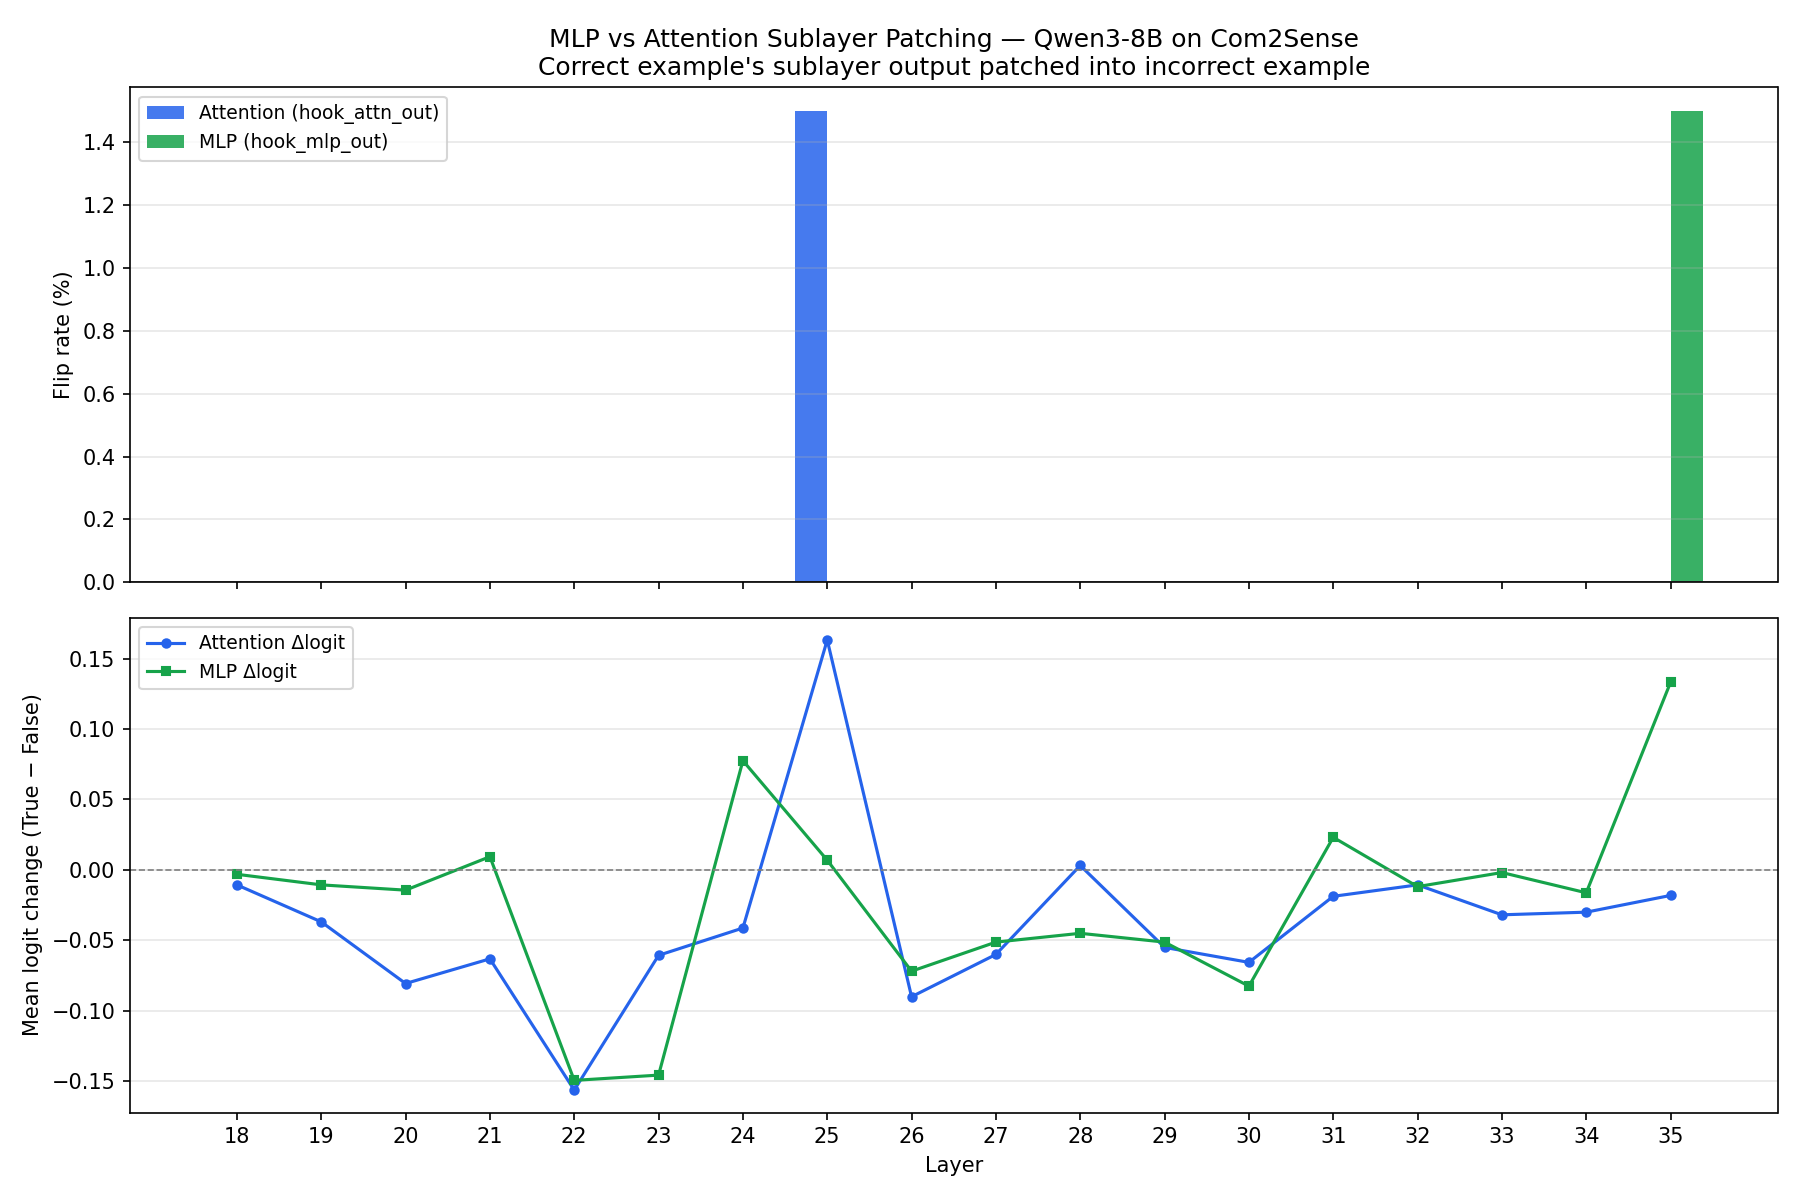
\includegraphics[width=\linewidth]{reports/figures/mlp_attn_patching.png}
\caption{MLP vs.\ attention sublayer patching results across all 18 layers. Unlike full-stream patching (Figure~\ref{fig:patching}), sublayer effects have mixed signs, revealing that the monotonically negative \texttt{resid\_post} results were an artifact of distributional mismatch rather than evidence of causal importance.}
\label{fig:mlp_attn}
\end{figure}

\begin{figure}[h]
\centering
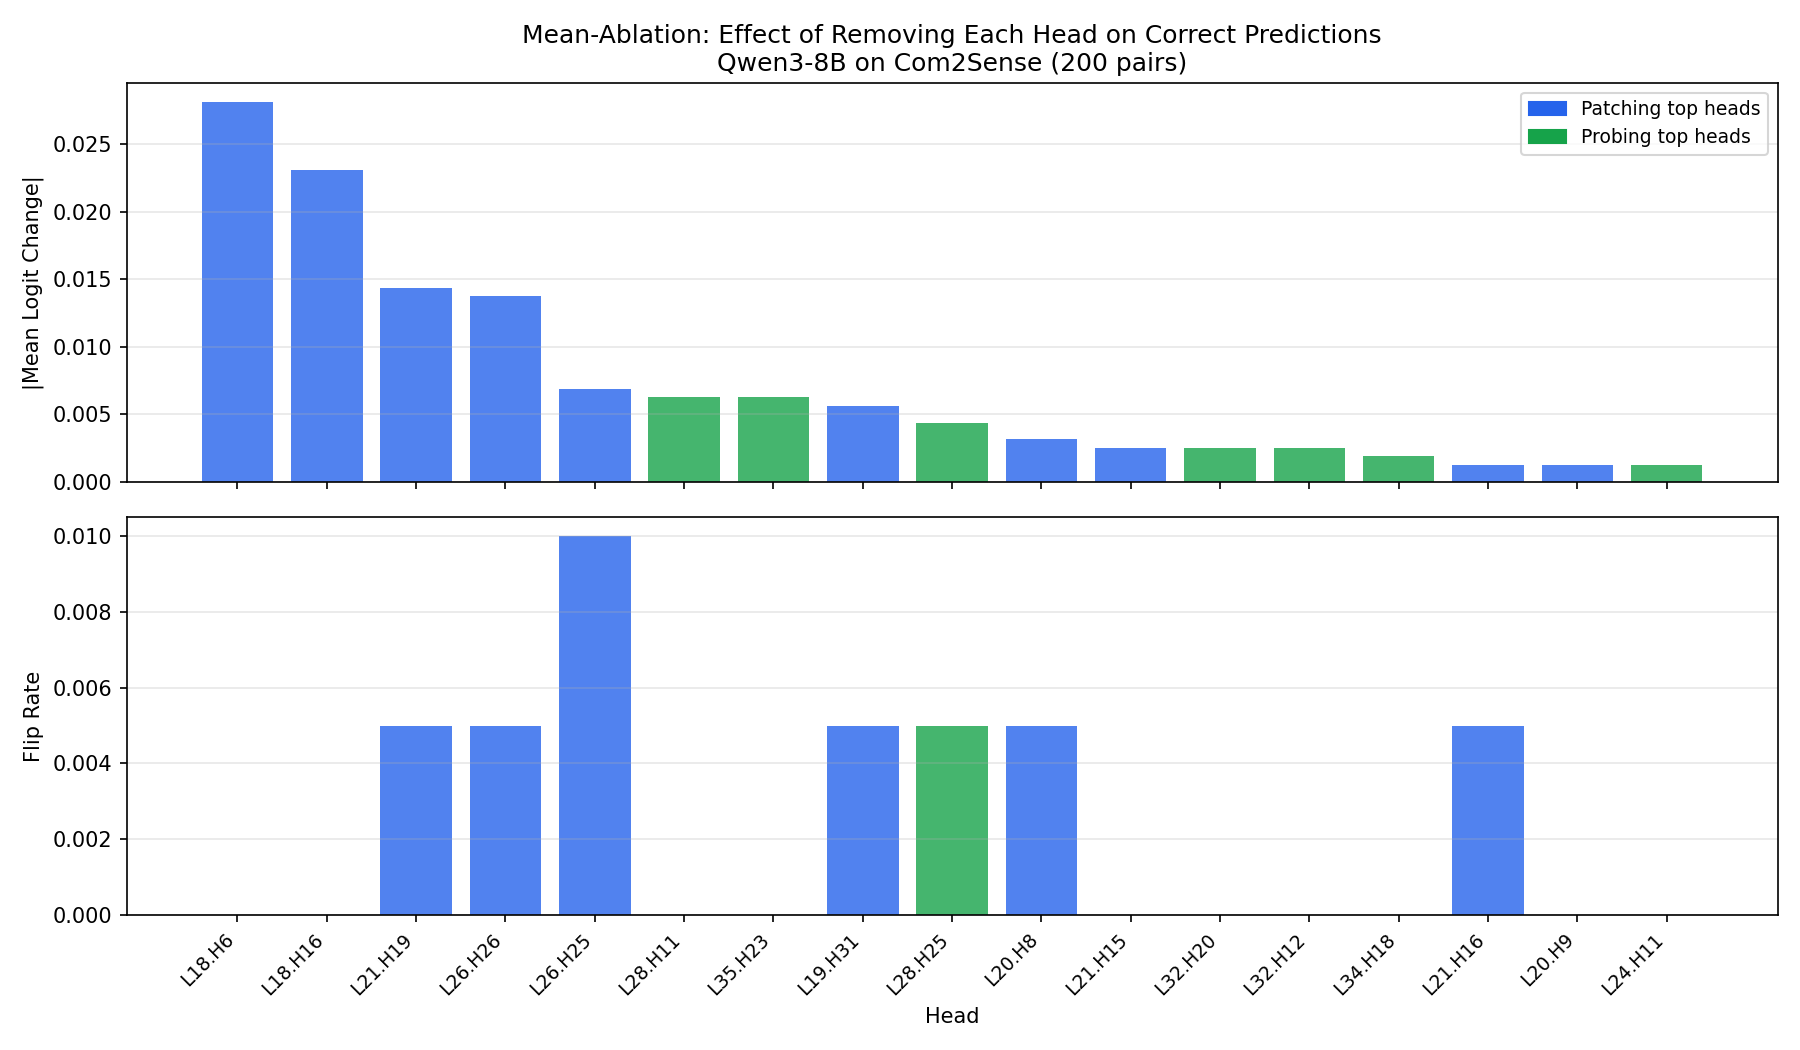
\includegraphics[width=0.75\linewidth]{reports/figures/ablation_results.png}
\caption{Mean-ablation flip rates for the 17 candidate attention heads. Maximum flip rate is 1.0\% (L26.H25, 2/200 correct predictions flipped). No head is necessary for correct commonsense predictions.}
\label{fig:ablation}
\end{figure}

\end{document}
